\title{Homework 3}
\author{Crist\'obal Armaza, Chris Silvia}
\date{\today}

\documentclass[11pt]{article}
\usepackage[letterpaper,left=2.2cm,right=2.2cm,top=2.2cm,bottom=2.5cm]{geometry}
\usepackage{graphicx}
\usepackage{hyperref}
\DeclareGraphicsExtensions{.bmp,.png,.jpg,.pdf}
\usepackage{amsmath}
\usepackage{courier}
\usepackage{natbib}
\usepackage{listings}
\linespread{1.2}

\newcommand{\Ma}{\text{Ma}}
\newcommand{\Rey}{\text{Re}}
\newcommand{\ind}[4]{{#1}^{#2}_{#3,#4}}
\newcommand{\fDx}[4]{\ind{#1}{#2}{#3+1}{#4} - \ind{#1}{#2}{#3}{#4}}
\newcommand{\bDx}[4]{\ind{#1}{#2}{#3}{#4} - \ind{#1}{#2}{#3-1}{#4}}
\newcommand{\fDy}[4]{\ind{#1}{#2}{#3}{#4+1} - \ind{#1}{#2}{#3}{#4}}
\newcommand{\bDy}[4]{\ind{#1}{#2}{#3}{#4} - \ind{#1}{#2}{#3}{#4-1}}
\newcommand{\cDxx}[4]{\ind{#1}{#2}{#3+1}{#4} - 2\ind{#1}{#2}{#3}{#4} + \ind{#1}{#2}{#3-1}{#4}}
\newcommand{\cDyy}[4]{\ind{#1}{#2}{#3}{#4+1} - 2\ind{#1}{#2}{#3}{#4} + \ind{#1}{#2}{#3}{#4-1}}
\newcommand{\cDxy}[4]{\ind{#1}{#2}{#3+1}{#4+1} - \ind{#1}{#2}{#3+1}{#4-1} - \ind{#1}{#2}{#3-1}{#4+1} + \ind{#1}{#2}{#3-1}{#4-1}}

\begin{document}
\maketitle

\section*{Organization}

We met to discuss the involved equations, as well as to figure how to efficiently handle the data for the code. We set up a Github repo to collaborate. Crist\'obal began the code, Chris also began the code in parallel, and then merged the progress Crist\'obal had made into his code to complete the code. With the code fully operating, Chris made the graphs to compare with Hou et al. (1995), while Crist\'obal made the streamline plots and finished the write up.

\section{Analytical Equations}

\subsection{Navier-Stokes for a compressible fluid}

We want to solve the continuity equation
\begin{equation}
\frac{\partial \rho}{\partial t} + \frac{\partial}{\partial x_k}\left(\rho u_k\right) = 0,
\end{equation}
and the momentum equation
\begin{equation}
\frac{\partial}{\partial t}\left(\rho u_i\right) + \frac{\partial}{\partial x_k}\left(\rho u_k u_i\right) = -\frac{\partial p}{\partial x_i} + \frac{\partial}{\partial x_k}\left[\mu\left(\frac{\partial u_i}{\partial x_k} + \frac{\partial u_k}{\partial x_i}- \frac{2}{3}\delta_{ik}\frac{\partial u_l}{\partial x_l}\right)\right],
\end{equation}
where we will assume the equation of state $p = c^2\rho$, $c$ being the speed of sound in the fluid. Note that the momentum equation can also be written in conservative form as
\begin{equation}
\frac{\partial}{\partial t}\left(\rho u_i\right) + \frac{\partial T_{ik}}{\partial x_k} = 0,
\end{equation}
where
\begin{equation}
T_{ik} := \rho u_i u_k + p\delta_{ik} - \mu\left(\frac{\partial u_i}{\partial x_k} + \frac{\partial u_k}{\partial x_i}- \frac{2}{3}\delta_{ik}\frac{\partial u_l}{\partial x_l}\right)
\end{equation}
is the stress-energy tensor.

%\subsection{Dimensionless Equations}

%Introducing a characteristic length scale $H$, velocity $U$, time $H/U$, and density $\rho_0$, we define the dimensionless quantities
%\begin{align}
%x &= H\tilde x,\\
%u_i &= U \tilde{u}_i,\\
%t &= \frac{H}{U}\,\tilde t,\\
%\rho &= \rho_0 \tilde\rho,\\
%p &= \rho c^2 = \rho_0 c^2 \tilde\rho
%\end{align}
%Plugging these definitions into both equations, assuming a constant viscosity, and dropping the tildes, we get the dimensionless equations
%\begin{equation}
%\frac{\partial \rho}{\partial t} + \frac{\partial}{\partial x_k}\left(\rho u_k\right) = 0,
%\end{equation}
%and 
%\begin{equation}
%\frac{\partial}{\partial t}\left(\rho u_i\right) + \frac{\partial T_{ik}}{\partial x_k} = 0,
%\end{equation}
%with
%\begin{equation}
%T_{ik} = \rho u_i u_k + \frac{1}{\Ma^2}\,\delta_{ik}\rho - \frac{1}{\Rey}\left(\frac{\partial u_i}{\partial x_k} + \frac{\partial u_k}{\partial u_i} - \frac{2}{3}\delta_{ik}\frac{\partial u_l}{\partial x_l}\right),
%\end{equation}
%where we introduced the Mach number, $\Ma = U/c$, and the Reynolds number, $\Rey = \rho_0 UH/\mu$.

\subsection{2-D Equations in Cartesian Equations}

Replacing $x_k = (x,y)$, $u_i = (u, v)$, we obtain
\begin{align}
T_{xx} &= \rho u^2 + c^2\rho - \frac{2\mu}{3}\left( 2\,\frac{\partial u}{\partial x} - \frac{\partial v}{\partial y} \right),\\
T_{yy} &= \rho v^2 + c^2\rho - \frac{2\mu}{3}\left( 2\,\frac{\partial v}{\partial y} - \frac{\partial u}{\partial x} \right),\\
T_{xy} = T_{yx} &= \rho u v - \mu\left( \frac{\partial u}{\partial y} + \frac{\partial v}{\partial x} \right),
\end{align}
and the equations we want to solve are
\begin{align}
\frac{\partial\rho}{\partial t} + \frac{\partial}{\partial x}\left(\rho u\right) + \frac{\partial}{\partial y}\left(\rho v\right) &= 0,\\
\frac{\partial}{\partial t}\left(\rho u\right) + \frac{\partial}{\partial x}\left( \rho u^2 + c^2\rho \right) + \frac{\partial}{\partial y}\left( \rho u v \right) - \mu\left(\frac{4}{3}\frac{\partial^2u}{\partial x^2} + \frac{1}{3}\frac{\partial^2 v}{\partial x \partial y} + \frac{\partial^2u}{\partial y^2}\right) &= 0,\\
\frac{\partial}{\partial t}\left( \rho v\right) + \frac{\partial}{\partial x}\left( \rho uv \right) + \frac{\partial}{\partial y}\left( \rho v^2 + c^2\rho\right) - \mu\left( \frac{\partial^2 v}{\partial x^2} + \frac{1}{3}\frac{\partial^2u}{\partial x \partial y} +  \frac{4}{3}\frac{\partial^2 v}{\partial y^2} \right) &= 0.
\end{align}
Here we have explicitly separated the hyperbolic part of each equation from the viscous (diffusive) terms. 

\section{Numerics}

\subsection{Finite Difference}

First off, we discretize the domain using a regular mesh in 2D over a finite amount of time:
\begin{align}
t_n = t_0 + n\,\Delta t_{n},\qquad n = 0,\hdots,n_t,\\
x_i = x_0 + i\,\Delta x,\qquad i = 0,\hdots,n_x-1,\\
y_j = y_0 + j\,\Delta x,\qquad j = 0,\hdots,n_y-1,
\end{align}
and set our coordinate system so that the left bottom corner is the origin, $x_0 = y_0 = 0$, and the simulation starts at $t_0 = 0$. The interval $\Delta t_{n}$ will be discussed later. Every physical quantity $\phi(t,x,y)$ is discretized as $\phi(t_n,x_i,y_j) = \ind{\phi}{n}{i}{j}$. On this mesh, we apply the MacCormack scheme for the hyperbolic part of each equation. To do so, these parts must be discretized using forward and backward schemes for the predictor and corrector steps, respectively. These discretizations read
\begin{align}
\phi'_i &= \frac{1}{\Delta x}\left(\phi_{i+1} - \phi_i \right) - \frac{\Delta x}{2}\phi''_i + \mathcal O(\Delta x^3),\\
\phi'_i &= \frac{1}{\Delta x}\left(\phi_i - \phi_{i-1} \right) + \frac{\Delta x}{2}\phi''_i + \mathcal O(\Delta x^3),
\end{align}
respectively. 

For the viscous term, we can just use a central scheme,
\begin{equation}
\phi''_i = \frac{1}{\Delta x^2}\left( \phi_{i+1} - 2\phi_i + \phi_{i-1} \right) - \frac{\Delta x^2}{12}\phi^{(iv)}_i + \mathcal O(\Delta x^4).
\end{equation}
The discretization for the cross derivative is a little less trivial. Recalling the central scheme for a first derivative,
\begin{equation}
\phi'_i = \frac{1}{2\,\Delta x}\left(\phi_{i+1} - \phi_{i-1}\right) - \frac{\Delta x^2}{6}\phi_i''' +  \mathcal O(\Delta x^4),
\end{equation}
we differentiate this with respect to $y$ to get
\begin{equation}
\left.\frac{\partial^2\phi}{\partial y \partial x}\right|_{i,j} = \frac{1}{2\,\Delta x}\left( \frac{\partial \phi_{i+1,j}}{\partial y} - \frac{\partial \phi_{i-1,j}}{\partial y} \right) - \frac{\Delta x^2}{6}\frac{\partial^4\phi}{\partial y\partial x^3} +  \frac{\partial}{\partial y}\mathcal O(\Delta x^4).
\end{equation}
Applying the same formula on all these terms (including the leading error term), and collecting terms, we arrive at
\begin{align}
\left.\frac{\partial^2\phi}{\partial y\partial x}\right|_{i,j} &= \frac{1}{4\,\Delta x\,\Delta y}\left( \phi_{i+1,j+1} - \phi_{i+1,j-1} - \phi_{i-1,j+1} + \phi_{i-1,j-1} \right)\\ 
&\quad- \frac{\Delta x^2}{6}\frac{\partial^4\phi}{\partial x^3\partial y} - \frac{\Delta y^2}{6}\frac{\partial^4\phi}{\partial x\partial y^3},
\end{align}
so we still have a second-order accurate discretization independently for each coordinate. Also, this expression clearly preserves the symmetry of cross derivatives.

\subsection{Expressions for Predictors and Correctors}

Replacing all the above finite difference expressions, we get
\begin{align}
\ind{\rho}{\star}{i}{j} &= \ind{\rho}{n}{i}{j} - a_1\left[ \fDx{(\rho u)}{n}{i}{j}\right] - a_2\left[ \fDy{(\rho v)}{n}{i}{j}\right],\\
\ind{(\rho u)}{\star}{i}{j} &= \ind{(\rho u)}{n}{i}{j} - a_1\left[ \fDx{(\rho u^2)}{n}{i}{j} + c^2\left(\fDx{\rho}{n}{i}{j}\right) \right] - a_2\left[ \fDy{(\rho u v)}{n}{i}{j} \right]\\
&\quad + \frac{4a_3}{3}\left[ \cDxx{u}{n}{i}{j} \right] + a_4\left[ \cDyy{u}{n}{i}{j} \right]\\
&\quad + a_5\left[ \cDxy{v}{n}{i}{j} \right],\\
\ind{(\rho v)}{\star}{i}{j} &= \ind{(\rho v)}{n}{i}{j} - a_1\left[ \fDx{(\rho u v)}{n}{i}{j} \right]- a_2\left[ \fDy{(\rho v^2)}{n}{i}{j} + c^2\left(\fDy{\rho}{n}{i}{j}\right) \right]\\
&\quad + a_3\left[ \cDxx{v}{n}{i}{j} \right] + \frac{4a_4}{3}\left[ \cDyy{v}{n}{i}{j} \right]\\
&\quad + a_5\left[ \cDxy{u}{n}{i}{j} \right]
\end{align}
for the predictor step, and
\begin{align}
\ind{\rho}{n+1}{i}{j} &= \frac{1}{2}\left[ \ind{\rho}{n}{i}{j} + \ind{\rho}{\star}{i}{j}\right] - \frac{a_1}{2}\left[ \bDx{(\rho u)}{\star}{i}{j}\right] - \frac{a_2}{2}\left[ \bDy{(\rho v)}{\star}{i}{j}\right],\\
\ind{(\rho u)}{n+1}{i}{j} &= \frac{1}{2}\left[ \ind{(\rho u)}{n}{i}{j} + \ind{(\rho u)}{\star}{i}{j} \right] - \frac{a_1}{2}\left[ \bDx{(\rho u^2)}{\star}{i}{j} + c^2\left(\bDx{\rho}{\star}{i}{j}\right) \right]\\
&\quad - \frac{a_2}{2}\left[ \bDy{(\rho u v)}{\star}{i}{j} \right] + \frac{2a_3}{3}\left[ \cDxx{u}{\star}{i}{j} \right]\\
&\quad + \frac{a_4}{2}\left[ \cDyy{u}{\star}{i}{j} \right] + \frac{a_5}{2}\left[ \cDxy{v}{\star}{i}{j} \right],\\
\ind{(\rho v)}{n+1}{i}{j} &= \frac{1}{2}\left[ \ind{(\rho v)}{n}{i}{j} + \ind{(\rho v)}{\star}{i}{j} \right] - \frac{a_2}{2}\left[ \bDy{(\rho v^2)}{\star}{i}{j} + c^2\left(\bDy{\rho}{\star}{i}{j}\right) \right]\\
&\quad - \frac{a_1}{2}\left[\bDx{(\rho u v)}{\star}{i}{j}\right] + \frac{a_3}{2}\left[ \cDxx{v}{\star}{i}{j} \right]\\
&\quad + \frac{2a_4}{3}\left[ \cDyy{v}{\star}{i}{j} \right] + \frac{a_5}{2}\left[ \cDxy{u}{\star}{i}{j} \right],
\end{align}
for the corrector step, where
\begin{equation}
a_1 = \frac{\Delta t}{\Delta x},\quad a_2 = \frac{\Delta t}{\Delta y},\quad a_3 = \frac{\mu\Delta t}{\Delta x^2},\quad a_4 = \frac{\mu\Delta t}{\Delta y^2},\quad a_5 = \frac{\mu\Delta t}{12\Delta x\,\Delta y}.
\end{equation}
These formulas are valid for interior points only. 

\subsection{Boundary Conditions}

Boundary conditions depend on the particular situation we are studying. For the lid-cavity problem with the sliding wall being the top boundary, the boundary conditions for the velocity are
\begin{align}
\ind{u}{n}{i}{0} &= 0,\, \ind{u}{n}{i}{n_y-1} = U\quad\text{for }i = 1,\hdots,(n_x-2),\\
\ind{u}{n}{0}{j} &= \ind{u}{n}{n_x-1}{j} = 0\quad \text{for }j = 0,\hdots,n_y-1,\\
\ind{v}{n}{i}{j} &= 0.
\end{align}
The boundary conditions for the density are trickier. They can be obtained from the continuity equation applied at every boundary. For example, for the boundary $x = 0$, $v = 0$ so $\partial(\rho v)/\partial y = 0$ there. Then, the continuity equation reads
\begin{equation}
\frac{\partial \rho}{\partial t} + \frac{\partial}{\partial x}\left(\rho u\right) = 0,\qquad (x = 0).
\end{equation}
In order to maintain second-order accuracy, we use a 3-point forward stencil
\begin{equation}
\phi_i' = \frac{-3\phi_i + 4\phi_{i+1} - \phi_{i+2}}{2\,\Delta x}
\end{equation}
to construct a MacCormack method at the boundary,
\begin{align}
\ind{\rho}{\star}{0}{j} &= \ind{\rho}{n}{0}{j} 
- \frac{a_1}{2}\left[-3\ind{(\rho u)}{n}{0}{j} + 4\ind{(\rho u)}{n}{1}{j} - \ind{(\rho u)}{n}{2}{j}\right],\\
\ind{\rho}{n+1}{0}{j} &= \frac{1}{2}\left[ \ind{\rho}{n}{0}{j} + \ind{\rho}{\star}{0}{j} \right] 
- \frac{a_1}{4}\left[-3\ind{(\rho u)}{\star}{0}{j} + 4\ind{(\rho u)}{\star}{1}{j} - \ind{(\rho u)}{\star}{2}{j}\right],
\end{align}
for $j = 1,\hdots,n_y-2$. Similarly, for the right wall ($x = (n_x-1)\Delta x$), we apply a 3-point backward stencil,
\begin{align}
\ind{\rho}{\star}{n_x-1}{j} &= \ind{\rho}{n}{n_x-1}{j} 
- \frac{a_1}{2}\left[\ind{(\rho u)}{n}{n_x-3}{j} - 4\ind{(\rho u)}{n}{n_x-2}{j} + 3\ind{(\rho u)}{n}{n_x-1}{j}\right],\\
\ind{\rho}{n+1}{n_x-1}{j} &= \frac{1}{2}\left[ \ind{\rho}{n}{n_x-1}{j} + \ind{\rho}{\star}{n_x-1}{j} \right] 
- \frac{a_1}{4}\left[\ind{(\rho u)}{\star}{n_x-3}{j} - 4\ind{(\rho u)}{\star}{n_x-2}{j} + 3\ind{(\rho u)}{\star}{n_x-1}{j}\right],
\end{align}
for $j = 1,\hdots,n_y-2$. Note that these two schemes do not include the points at the four corners; they deserve special attention. For the bottom, $u = 0$ and thus $\partial(\rho u)/\partial x = 0$, so
\begin{align}
\ind{\rho}{\star}{i}{0} &= \ind{\rho}{n}{i}{0} - \frac{a_2}{2}\left[ -3\ind{(\rho v)}{n}{i}{0} + 4\ind{(\rho v)}{n}{i}{1} - \ind{(\rho v)}{n}{i}{2} \right],\\
\ind{\rho}{n+1}{i}{0} &= \frac{1}{2}\left[\ind{\rho}{n}{i}{0} + \ind{\rho}{\star}{i}{0}\right] - \frac{a_2}{4}\left[ -3\ind{(\rho v)}{\star}{i}{0} + 4\ind{(\rho v)}{\star}{i}{1} - \ind{(\rho v)}{\star}{i}{2} \right].
\end{align}
for $i = 1,\hdots,n_x-2$. For the top, $u = U$ so $\partial(\rho u)/\partial x = U\partial \rho/\partial x$. Thus,
\begin{align}
\ind{\rho}{\star}{i}{n_y-1} &= \ind{\rho}{n}{i}{n_y-1} - \frac{a_1 U}{2}\left[\ind{\rho}{n}{i+1}{n_y-1} - \ind{\rho}{n}{i-1}{n_y-1}\right] - \frac{a_2}{2}\left[ \ind{(\rho v)}{n}{i}{n_y - 3} - 4\ind{(\rho v)}{n}{i}{n_y - 2} + 3\ind{(\rho v)}{n}{i}{n_y-1} \right],\\
\ind{\rho}{n+1}{i}{n_y-1} &= \frac{1}{2}\left[\ind{\rho}{n}{i}{n_y-1} + \ind{\rho}{\star}{i}{n_y-1} \right] - \frac{a_1 U}{4}\left[\ind{\rho}{\star}{i+1}{n_y-1} - \ind{\rho}{\star}{i-1}{n_y-1}\right]\\
&\quad- \frac{a_2}{4}\left[ \ind{(\rho v)}{\star}{i}{n_y - 3} - 4\ind{(\rho v)}{\star}{i}{n_y - 2} + 3\ind{(\rho v)}{\star}{i}{n_y-1} \right],
\end{align}
for $i = 1,\hdots,(n_x-2)$. Note that for $\partial\rho/\partial x$ we use a central stencil, which is also second-order accurate. Finally, for each corner, one notes that there are two available formulas provided by the above conditions.
We simple take the conditions determined by the left and right sides, respectively.

\subsection{System Ready to Be Solved!}

In summary, our grid consists of $n_x \times n_y$ points, out of which $2(n_y - 2) + 2(n_x -2) + 4$ are determined by boundary conditions. The other $n_x \times n_y - 2n_y - 2n_x + 4 = (n_x - 2)(n_y - 2)$ points are determined by the $(n_x - 2)(n_y - 2)$ equations for the interior points.

\subsection{Initial Conditions}

We took uniform density everywhere and zero momentum (except at the top boundary, where there is the velocity $U$) as initial conditions.

\subsection{Stability}

We took the God-given formula
\begin{equation}
 \Delta t \leq \frac{\sigma}{1 + 2\,/\Rey_\Delta}\left[ \frac{U}{\Delta x} + \frac{U}{\Delta y} + c\sqrt{\frac{1}{\Delta x^2} + \frac{1}{\Delta y^2}} \right]^{-1},
\end{equation}
where $\sigma \leq 1$ is a safety parameter, which is arbitrary, and $\Rey_\Delta = \text{min}(\rho\Delta x|u|/\mu, \rho\Delta y|v|/\mu)$, where the values in bar are understood to be
the maximum values over the domain.


\section{Results}

\subsection{Comparison with Hou et al. (1995)}

Figure \ref{Central Profile} shows the $u$ velocity along the center line of the simulation region, at $x=H/2$, and compares it to Hou et al., who determined the velocity using a lattice boltzmann method.  We see that there is good agreement with Hou's profile, in both the qualitative shape, and the approximate location of the transition from negative to positive velocities.

\begin{center}
\begin{figure}[ht!]
\begin{minipage}{16cm}\label{Central Profile}
\includegraphics[width=8cm]{hou_cropped}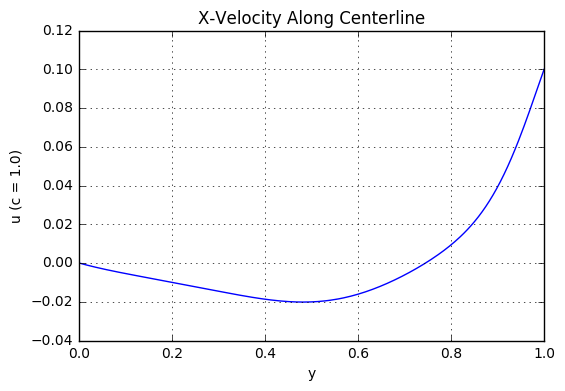
\includegraphics[width=8cm]{u_profile}
\end{minipage}
\caption{Central Streamline, compared to Hou et al. (1995).  Recall for us, $Re=100$.}
\end{figure}
\end{center}

\subsection{Streamlines}

Figure \ref{streamlines} show the streamlines for different timesteps during the evolution. In these plots, $\Rey = 100$ and the color code indicates the speed of the flow, defined as $\sqrt{u^2 + v^2}$. Starting from the initial condition of zero momentum, we observe the formation of a primary circulating eddy, which induces the formation of two secondary counter-rotating eddies at the bottom corners. This is in agreement with Hou et al. (1995) and the results analyzed there. By the end of the simulation, we confirm that the flow pattern remains stable in time, presenting the steady flow shown in Fig. \ref{steady}. For comparison, we also include the result from Hou et al., finding a remarkable agreement between both results.

\begin{center}
\begin{figure}[ht!]
\begin{minipage}{16cm}\label{streamlines}
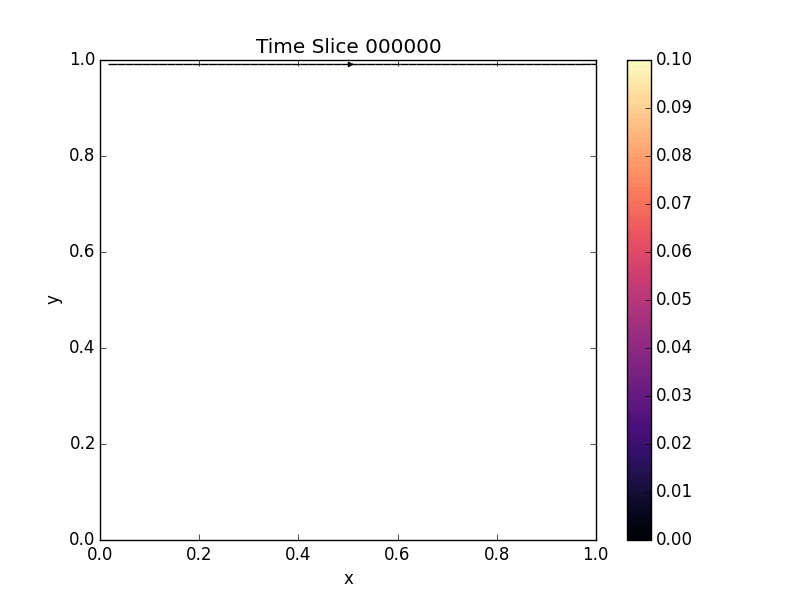
\includegraphics[width=8cm]{seq01}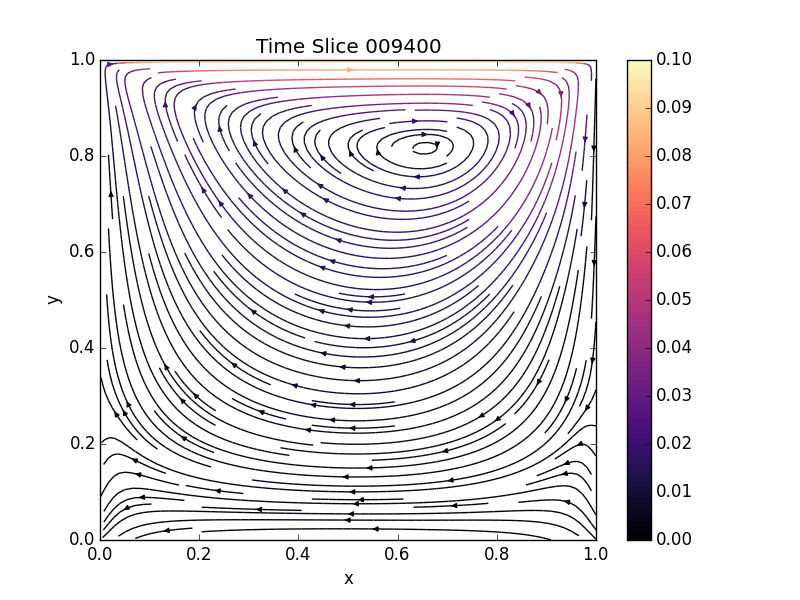
\includegraphics[width=8cm]{seq02}
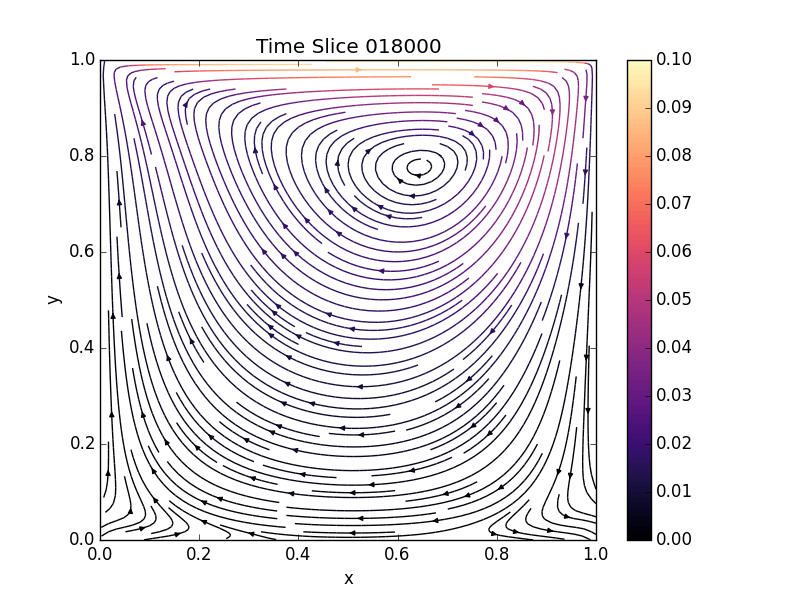
\includegraphics[width=8cm]{seq03}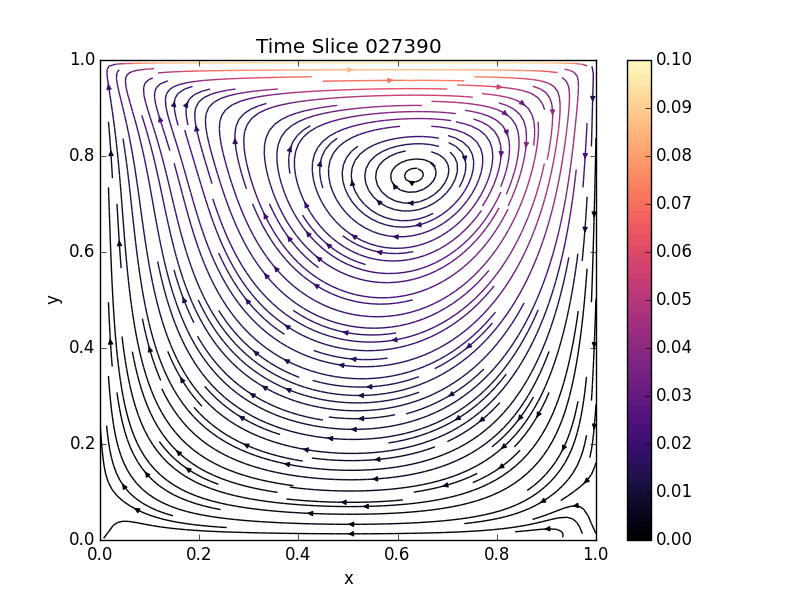
\includegraphics[width=8cm]{seq04}
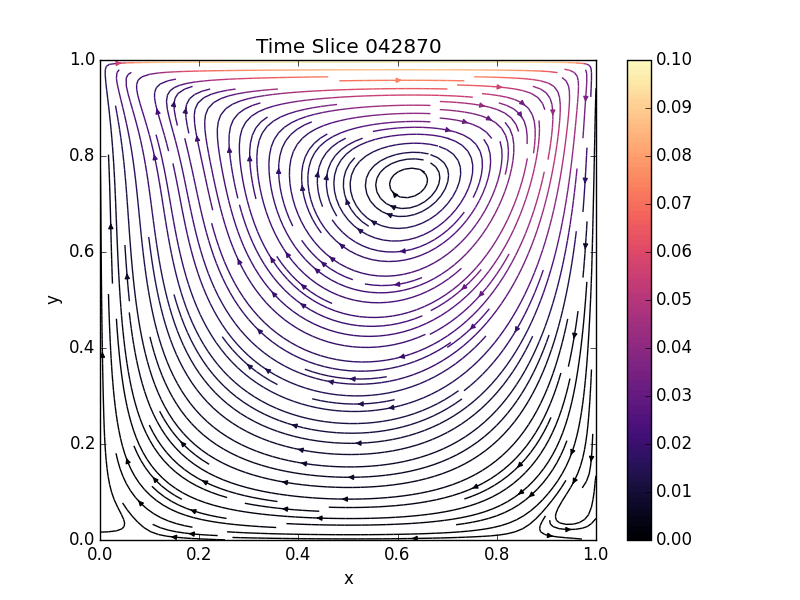
\includegraphics[width=8cm]{seq05}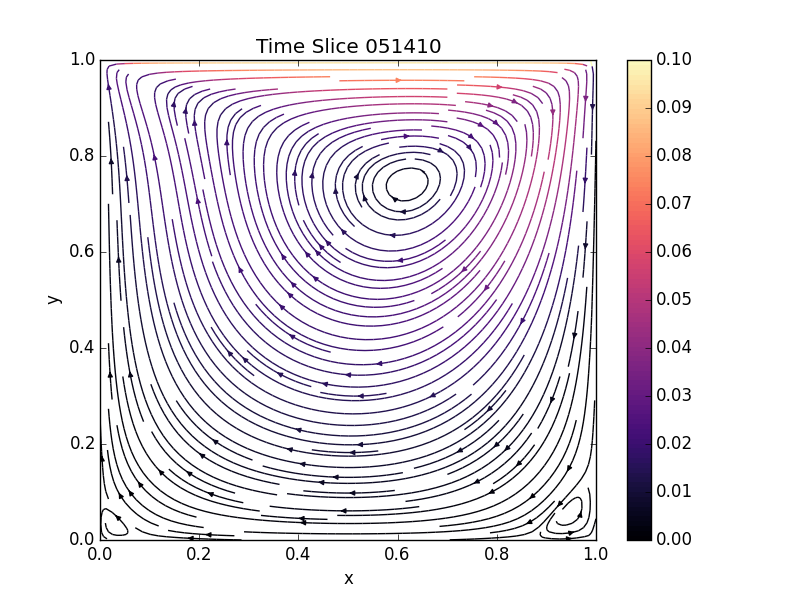
\includegraphics[width=8cm]{seq06}
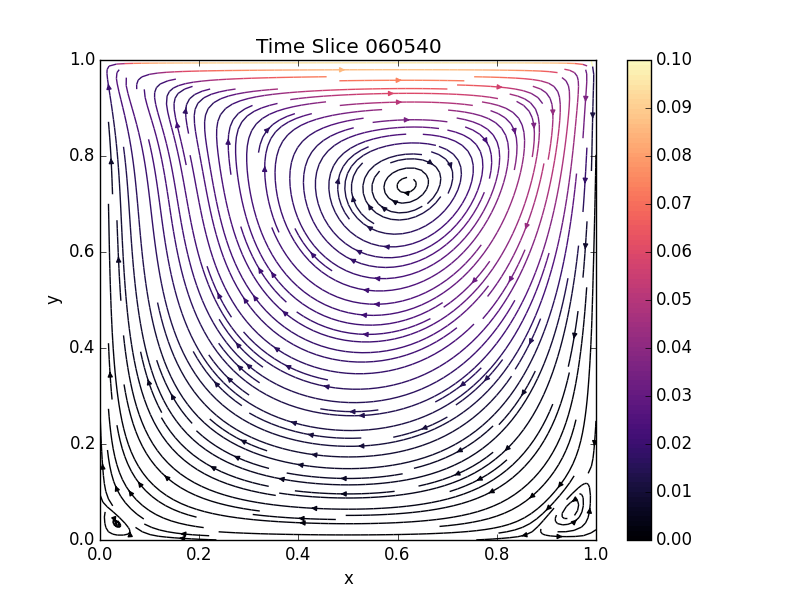
\includegraphics[width=8cm]{seq07}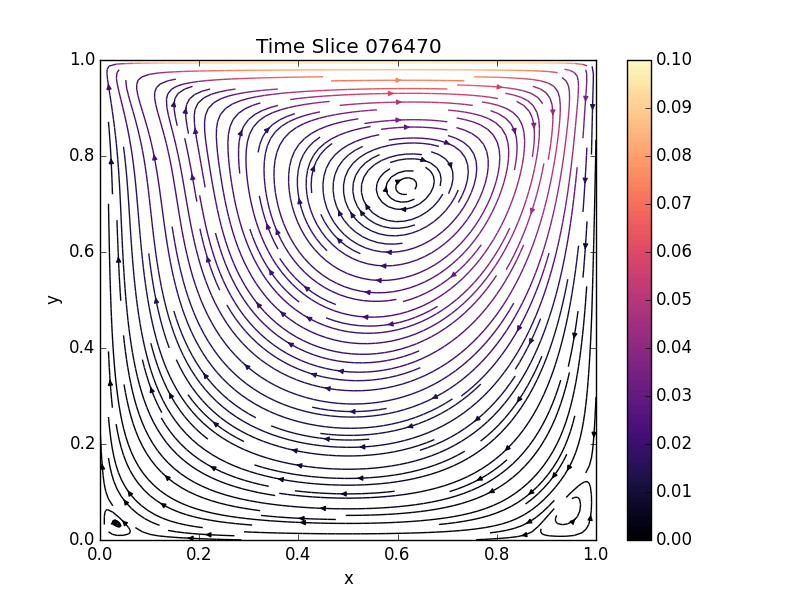
\includegraphics[width=8cm]{seq08}
\end{minipage}
\caption{Streamlines at different times.}
\end{figure}
\end{center}

\begin{center}
\begin{figure}[ht!]
\begin{minipage}{16cm}\label{steady}
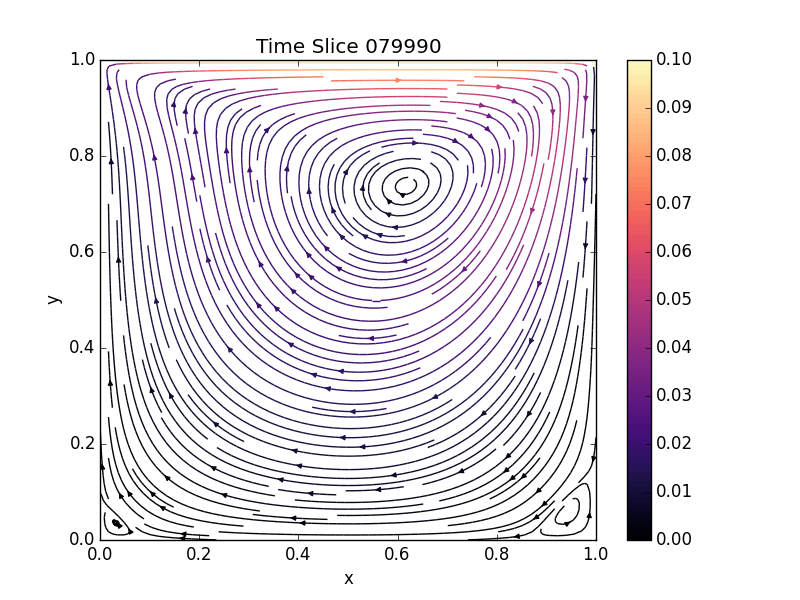
\includegraphics[width=9cm]{final}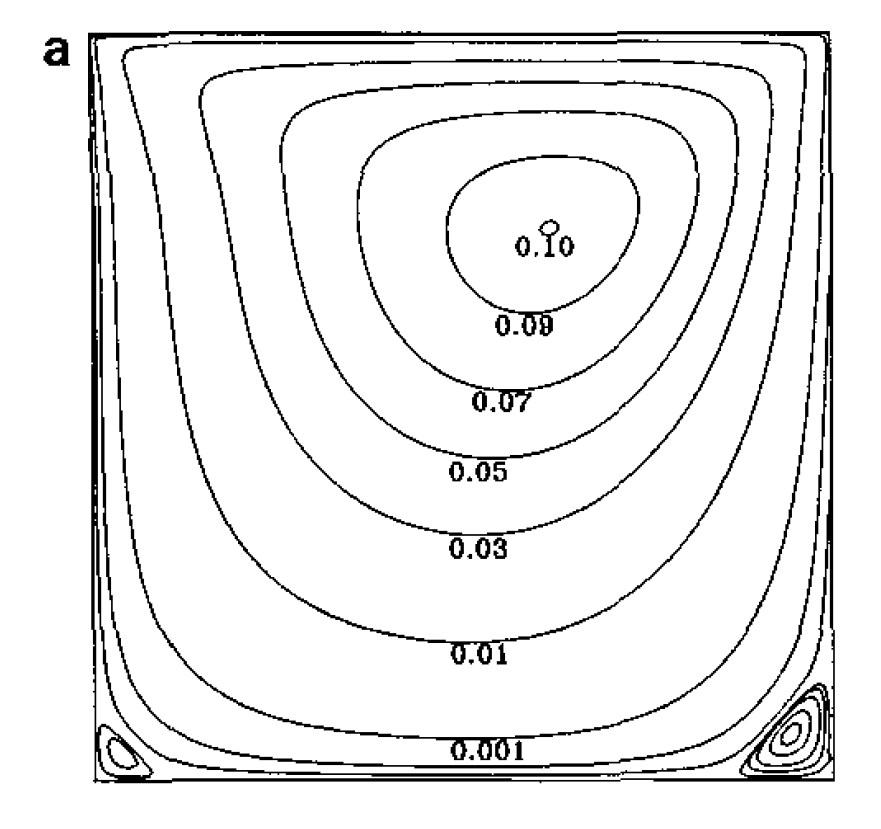
\includegraphics[width=6.5cm]{HouStreamlines}
\end{minipage}
\caption{Steady state. Comparison with Hou et al. (1995)}
\end{figure}
\end{center}

\appendix
\section{Code}

\lstinputlisting[language=c++]{csv_generator.cpp}

\end{document}
